\section{Benchmarks de l'approche génétique}

Il s'agira dans cette partie d'évaluer le temps que met notre approche génétique en fonction des paramètres d'entrée. Il peut en effet être intéressant de savoir si notre algorithme évolue de façon linéaire ou exponentielle par rapport à ces derniers.

Le fichier de données considéré correspond au \textit{Barnes - setb4c9}. En effet, il comporte $15$ jobs et $11$ machines ce qui le rend intéressant de par la taille du problème.

Le code servant à réaliser les benchmarks est disponible dans le fichier \textit{benchmarks.py}.

\subsection{Comparaison du temps d'exécution par rapport à la taille de la population}

La génération maximale est ici fixée à $100$. Nous faisons évoluer la taille de la population de façon logarithmique entre $1$ et $1000$.

\begin{figure}[!h]
    \centering
    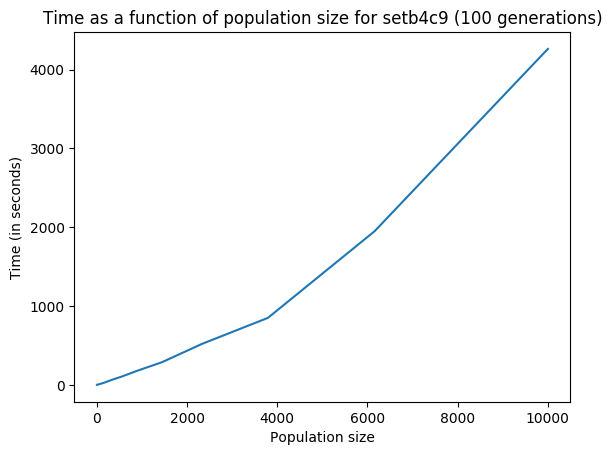
\includegraphics[]{report/Pictures/setb4c9_benchmarks_population.png}
\end{figure}

A $max\_generation$ fixé, le temps de calcul est linéaire en fonction du nombre d'individus dans la population.

\subsection{Comparaison du temps d'exécution par rapport à la génération maximale}

La taille de la population est ici fixée à $100$. Nous faisons évoluer la génération maximale de façon logarithmique entre $1$ et $1000$.

\begin{figure}[!h]
    \centering
    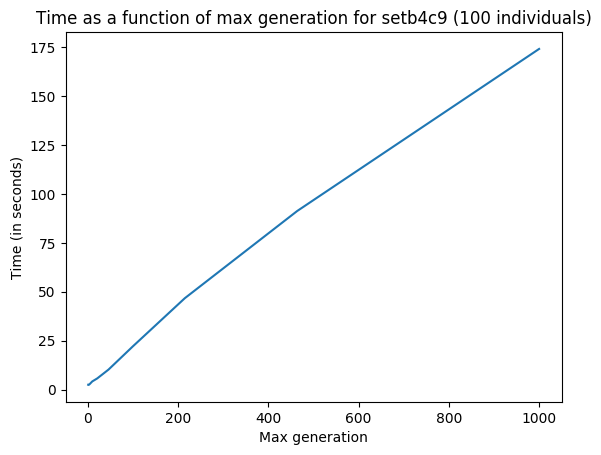
\includegraphics[]{report/Pictures/setb4c9_benchmarks_generation.png}
\end{figure}

A $population\_size$ fixé, le temps de calcul est linéaire en fonction de la génération maximale.

\newpage

\subsection{Comparaison du temps d'exécution par rapport à la taille de la population et la génération maximale}

\begin{figure}[!h]
    \centering
    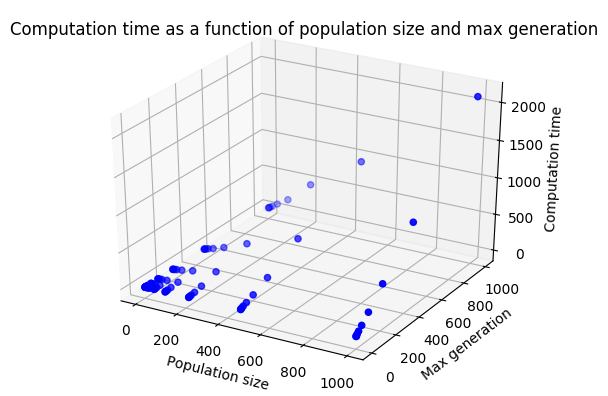
\includegraphics[]{report/Pictures/setb4c9_benchmarks_generation_with_computation_time.png}
\end{figure}

\newpage

\subsection{Comparaison de la fonction objective par rapport à la taille de la population et la génération maximale}

\begin{figure}[!h]
    \centering
    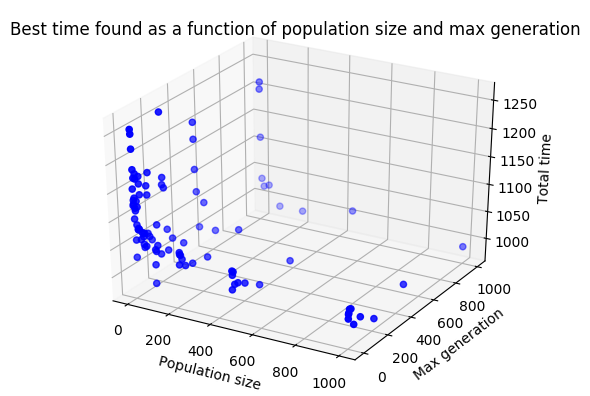
\includegraphics[]{report/Pictures/setb4c9_benchmarks_generation_with_solution_time.png}
\end{figure}

